\documentclass[aspectratio=169]{beamer}
\usetheme{focus}

%\usepackage{beamerthemesplit}
%\beamertemplatenavigationsymbolsempty
\usepackage{amsmath}
\usepackage{amsthm}
\usepackage{amssymb}
\usepackage{latexsym}
\usepackage{graphicx}
\usepackage{fancybox}
\usepackage{dsfont}
\usepackage{multirow} 
\usepackage{multicol}
\usepackage{booktabs} 
\usepackage{dcolumn}
\usepackage{soul}
\usepackage[cache=false]{minted}
\usepackage{MnSymbol}
\usepackage{stmaryrd}


\DeclareMathOperator*{\argmax}{arg\,max}
\DeclareMathOperator*{\argmin}{arg\,min}

\newcommand{\X}{\mathtt{X}}
\newcommand{\Y}{\mathtt{Y}}

%\newcommand{\R}{\mathbb{R}}
%\newcommand{\E}{\mathbb{E}}
%\newcommand{\V}{\mathbb{V}}
\newcommand{\p}{\mathbb{P}}
\newcommand*\df{\mathop{}\!\mathrm{d}}
\newcommand{\del}{\partial}


% imports
\usepackage{xargs}
\usepackage{xpatch}
\usepackage{etoolbox}
\usepackage{pdflscape}
\usepackage{booktabs}
\usepackage{threeparttable}
\usepackage[skip=0.2\baselineskip]{caption}

% command for inputting raw latex
\makeatletter
\newcommand\primitiveinput[1]{\@@input #1 }
\makeatother

% common table command
\newcommandx{\tablecontent}[4]{
    \begin{threeparttable}[!ht]
        \centering
        \caption{#3}
        \vspace{-1em}
        \footnotesize
        \begin{tabular}{#1}
            \primitiveinput{../tables/#2.tex}
        \end{tabular}
        \vspace{-0.2em}
        \begin{tablenotes}[flushleft]
            #4
        \end{tablenotes}
    \end{threeparttable}
}




% \usepackage{slashbox}
\title{Lecture 4: Bayesian Analysis}
\author{Chris Conlon }
\institute{NYU Stern }


\newcommand{\norm}[1]{\left\lVert#1\right\rVert}
\newcommand{\R}{\mathbb{R}}
\newcommand{\E}{\mathbb{E}}
\newcommand{\V}{\mathbb{V}}
\newcommand{\ol}{\overline}
%\newcommand{\ul}{\underline}
\newcommand{\pp}{{\prime \prime}}
\newcommand{\ppp}{{\prime \prime \prime}}
\newcommand{\policy}{\gamma}


\newcommand{\fp}{\frame[plain]}

\date{\today}

\begin{document}
\maketitle


\begin{frame}{Quick Refresh: Bayes Rule}
\begin{align*}
P(A | B)=\frac{P(B | A) P(A)}{P(B)}
\end{align*}
Given a \alert{positive test result} what is the probability a patient actually has cancer?
\begin{center}
\begin{table}[htp]
\caption{Test Accuracy}
\begin{center}
\begin{tabular}{l|r|r|}
& Cancer (1\%) & No Cancer (99\%) \\ \toprule
Positive Test& 80\% & 9.6\% \\
Negative Test& 20\% & 90.4\%
\end{tabular}
\end{center}
\end{table}%
\end{center}
\end{frame}


\begin{frame}{Quick Refresh: Bayes Rule}
Caclulate $Pr(Cancer \& Positive Test)$ and $Pr(No Cancer \& Positive Test)$
\begin{center}
\begin{table}[htp]
\caption{Joint Probabilities}
\begin{center}
\begin{tabular}{l|r|r|}
& Cancer (1\%) & No Cancer (99\%) \\ \toprule
Positive Test& (0.8)(0.01)=0.008 & (0.9)(0.096)=0.09504 \\
Negative Test& (0.2)(0.01)=0.002 & (0.9)(0.904)=0.89496
\end{tabular}
\end{center}
\end{table}
\end{center}
$Pr(Cancer | Positive Test) = \frac{Pr(Cancer, Pos Test)}{Pr(Cancer,Pos Test) + Pr(NoCancer, Pos Test)}= .008/.10304 = 0.0776$
\end{frame}



\begin{frame}{Introduction}
\begin{itemize}
\item Suppose that we toss a coin several times with $x_i \in \{H,T\}=\{1,0\}$ 
\item $\mathbf{X} = \{H,T,H,H,\ldots\}$.
\item Suppose that the probability of heads $Pr(x_i = H) = p$.
\item What is the likelihood of an observed sequence of $\mathbf{X}$? where $x_i$ are I.I.D.
\begin{align*}
Pr(x_i | p) &= p^{x_i} (1-p)^{1-x_i} \\
Pr(\mathbf{X} | p) &=  p^{\sum_i x_i} (1-p)^{\sum_i (1- x_i)} 
\end{align*}
\end{itemize}
\end{frame}

\begin{frame}{Introduction: MLE for coin toss}
Can construct the \alert{log likelihood} and find the MLE.
\begin{align*}
\ell(\mathbf{X} | p) &= (\sum_i  x_i ) \ln p + (N-\sum_i x_i) \ln (1-p)\\
\frac{\partial \ell(p) }{\partial p} &= (\sum_i  x_i ) \frac{1}{p} - (N-\sum_i x_i) \frac{1}{1-p} =0\\
\frac{1-p}{p}  &= \frac{(\frac{1}{N}\cdot N-\frac{1}{N}\cdot\sum_i x_i) }{\frac{1}{N}\cdot \sum_i x_i} \rightarrow \hat{p} = \frac{1}{N}\cdot \sum_i x_i
\end{align*}
\end{frame}


\begin{frame}{Introduction: MLE for coin toss}
Can also construct the properties of $\hat{p}$.
\begin{align*}
\mathbb{E}[\hat{p}] &= \mathbb{E} \left[ \frac{1}{N}\cdot \sum_i x_i \right]  = \left[ \frac{1}{N}\cdot \sum_i \mathbb{E} x_i \right]  = \mu_x = p_0\\
\mathbb{V}[\hat{p} | \mathbf{X}] &= \mathbb{V} \left[ \frac{1}{N}\cdot \sum_i x_i \right]  =  \frac{1}{N^2}\cdot \sum_i \mathbb{V} (x_i ) = \frac{N}{N^2} p (1-p)
\end{align*}
Which gives us a CI of:  $\left(\overline{x} \pm 1.96 \cdot \sqrt{\frac{1}{N} \overline{x} (1-\overline{x})} \right)$
\end{frame}

\begin{frame}{Bayesian Statistics: Brief Introduction}
A different idea:
\begin{itemize}
\item Start with a (diffuse) initial guess for the distribution of $p$: $f_P(p)$.
\item Incorporate information from likelihood: $f(x_i | p)$
\item Construct \alert{posterior density} estimate $f(p | x_i)$.
\begin{itemize}
\item This doesn't characterize a best estimate $\hat{p}$ but a full distribution.
\item We can calculate $\mathbb{E}[p | x_i]$ or $\mathbb{V}[p |x_i]$ or any other functions of the posterior density.
\end{itemize}
\item Challenge: How to choose initial $f_P(p)$.
\end{itemize}
\end{frame}



\begin{frame}{Bayesian Statistics: Brief Introduction}
One possible guess is the uniform distribution $f(x) = 0$ on $0 \leq x \leq 1$.
\begin{itemize}
\item \alert{Marginal/Prior Distribution}: $f_P(p) = 1$ for $0 \leq p \leq 1$.
\item \alert{Conditional Distribution}/Likelihood: $f_{X|P} (x | p) = p^x (1-p)^{1-p}$
\item \alert{Joint Distribution} : $f_{X,P}(x, p)=f_{X|P}(x | p)\cdot f_P(p)  = p^x (1-p)^{1-p}\cdot 1 = x \cdot p + (1-x) \cdot (1-p)$
\begin{itemize}
\item This is only defined for $p \in[0,1]$ and $x \in \{0,1\}$. It is zero elsewhere.
\end{itemize}
\item What about \alert{Marginal Distribution} for $x$?
\begin{align*}
\int _ { p } f _ { P X } ( x , p ) d p &= x \cdot \int _ { 0 } ^ { 1 } p d p + ( 1 - x ) \cdot \int _ { 0 } ^ { 1 } ( 1 - p ) d p \\
&= x \cdot \frac { 1 } { 2 } + ( 1 - x ) \cdot \frac { 1 } { 2 } = \frac { 1 } { 2 } \propto 1
\end{align*}
\end{itemize}
\end{frame}


\begin{frame}{Bayesian Statistics: Brief Introduction}
The object we are usually interested in is the \alert{Posterior Distribution}
\begin{align*}
f _ { P | X } ( p | x ) = \frac { f _ { X | P } ( x | p ) \cdot f _ { P } ( p ) } { \int _ { 0 } ^ { 1 } f _ { X | P } ( x | p ) \cdot f _ { P } ( p ) d p } = 2 p ^ { x } ( 1 - p ) ^ { 1 - x } \propto p ^ { x } ( 1 - p ) ^ { 1 - x }
\end{align*}
\begin{itemize}
\item We are back at the p.m.f. of the \alert{Bernoulli} which is maybe comforting.\\
\item This is true because $f_X(x) \propto 1$ and $f_P(p) \propto 1$.
\item $f _ { P | X } ( p | x=0) = (1-p)$ and $f _ { P | X } ( p | x =1)=p$.
\end{itemize}
\end{frame}

\begin{frame}{Bayesian Statistics: Beta-Prior}
\begin{itemize}
\item Let's try a different \alert{prior distribution} than the uniform we used last time. This time we will use a $Beta(\alpha,\beta)$ distribution:
\begin{align*}
f _ { P } ( p | \alpha,\beta) &= \frac { \Gamma ( \alpha + \beta ) } { \Gamma ( \alpha ) \cdot \Gamma ( \beta ) } p ^ { \alpha - 1 } ( 1 - p ) ^ { \beta - 1 }\\
\mathbb{E}[p | \alpha,\beta] &=\frac{\alpha}{\alpha + \beta}\\
\mathbb{V}[p | \alpha,\beta] &=\frac{\alpha \beta}{(\alpha + \beta)^2(\alpha+\beta+1)}
\end{align*}
\item This has the advantage that it places nicely with the Binomial.
\item Consider $\alpha=16, \beta=8$. This gives $\mathbb{E}[p ] = \frac{2}{3}$ and $\mathbb{SE}[p] = 0.094$. 
\end{itemize}
\end{frame}


\begin{frame}{Bayesian Statistics: Beta-Prior}
Consider the case where $x=1$ (we get one piece of new data).
\begin{align*}
f _ { P } ( p ) \cdot f _ { X | P } ( x | p ) =\underbrace{ \frac { \Gamma ( \alpha + \beta ) } { \Gamma ( \alpha ) \cdot \Gamma ( \beta ) }}_{C(\alpha,\beta)} p ^ { \alpha - 1 } ( 1 - p ) ^ { \beta - 1 } \cdot p \propto  p ^ { \alpha  } ( 1 - p ) ^ { \beta - 1 } 
\end{align*}
\begin{itemize}
\item The resulting distribution is now $(p|x=1)\sim Beta(\alpha+1,\beta)$.
\item Our posterior has mean $=0.68$ and SE $=0.091$.
\item Estimate of mean increases and SE decreases.
\item Likewise if $x=0$ we get $(p|x=0)\sim Beta(\alpha,\beta+1)$
\item There is a \alert{conjugacy} relationship between the Beta and the Binomial.
\end{itemize}
\end{frame}



\begin{frame}{General Case}
\begin{align*}
\overbrace{f_{\theta|X}(\theta | x)}^{\text{posterior}}=\frac{\overbrace{f_{X, \theta}(x, \theta)}^{\text{joint}}}{ \underbrace{f_{X}(x)}_{\text{marginal of } x}}
=\frac{\overbrace{f_{X|\theta}(x | \theta)}^{\text{likelihood}} \cdot  \overbrace{f_{\theta}(\theta)}^{\text{prior}}}{\int f_{X|\theta}(x | \theta) \cdot f_{\theta}(\theta) d \theta}
\end{align*}
There is a shortcut because the denominator doesn't depend on $\theta$
\begin{align*}
f_{\theta|X}(\theta | x) \propto f_{X|\theta}(x | \theta) \cdot f_{\theta}(\theta)=\mathcal{L}(\theta | x) \cdot f_{\theta}(\theta)
\end{align*}
We can cheat because there exists a constant $c$ so that $c \int \mathcal{L}(\theta | x) \cdot f_{\theta}(\theta) d \theta=1$.
\end{frame}

\begin{frame}{A Normal Example}
Assume $X \sim N(\mu,1)$ and $\mu \sim N(0,100)$. What is $f_{\mu | X}(\mu | X=x)$?
\begin{align*}
f_{\mu|X}(\mu | x) &\propto \exp \left(-\frac{1}{2}(x-\mu)^{2}\right) \cdot \exp \left(-\frac{1}{2 \cdot 100} \mu^{2}\right)\\
&=\exp -\frac{1}{2} (x^{2}-2 x \mu+\mu^{2}+\mu^{2} / 100) \\
&\propto \exp \left(-\frac{1}{2(100 / 101)}(\mu-(100 / 101) x)^{2}\right)
\end{align*}
It happens that $(u | x) \sim N(100x/101 , 100/101)$. \\
In general the posterior will not be well defined.
\end{frame}

\begin{frame}{Kalman Update: A More Complicated Normal}
Assume $X \sim N(\mu,\sigma^2)$ with $\sigma^2$ known. $\mu \sim N(\mu_0,\tau^2)$. What is $f_{\mu | X}(\mu | X=x)$?
\begin{align*}
f_{\mu|X}(\mu | x) &\propto \exp \left(-\frac{1}{2 \sigma^{2}}(x-\mu)^{2}\right) \cdot \exp \left(-\frac{1}{2 \cdot \tau^{2}}\left(\mu-\mu_{0}\right)^{2}\right)\\
&\propto \exp -\frac{1}{2}\left(\frac{x^{2}}{\sigma^{2}}-\frac{2 x \mu}{\sigma^{2}}+\frac{\mu^{2}}{\sigma^{2}}+\frac{\mu^{2}}{\tau^{2}}-\frac{2 \mu \mu_{0}}{\tau^{2}}+\frac{\mu_{0}^{2}}{\tau^{2}}\right)\\
&\propto \exp -\frac{1}{2}\left(\mu^{2} \frac{\sigma^{2}+\tau^{2}}{\tau^{2} \sigma^{2}}-\mu \frac{2 x \tau^{2}+2 \mu_{0} \sigma^{2}}{\tau^{2} \cdot \sigma^{2}}\right)\\
&\propto \exp -\frac{1}{2\left(1 /\left(1 / \tau^{2}+1 / \sigma^{2}\right)\right)}\left(\left(\mu-\left(x / \sigma^{2}+\mu_{0} / \tau^{2}\right) /\left(1 / \sigma^{2}+1 / \tau^{2}\right)\right)\right.
\end{align*}
The resulting distribution is Normal with mean and variance
\begin{align*}
\mathbb{E}[\mu | X=x]=\frac{\frac{x}{\sigma^{2}}+\frac{\mu_{0}}{\tau^{2}}}{\frac{1}{\sigma^{2}}+\frac{1}{\tau^{2}}}, \quad \frac{1}{\mathbb{V}(\mu | X)}=\frac{1}{\sigma^{2}}+\frac{1}{\tau^{2}}
\end{align*}
\end{frame}


\begin{frame}{Kalman Update: A More Complicated Normal}
Despite being a giant mess this makes sense:
\begin{align*}
\mathbb{E}[\mu | X=x]=\frac{\frac{x}{\sigma^{2}}+\frac{\mu_{0}}{\tau^{2}}}{\frac{1}{\sigma^{2}}+\frac{1}{\tau^{2}}}, \quad \frac{1}{\mathbb{V}(\mu | X)}=\frac{1}{\sigma^{2}}+\frac{1}{\tau^{2}}
\end{align*}
\begin{itemize}
\item Posterior mean is a weighted average of \alert{prior mean} and \alert{sample mean}.
\item Weights depend on \alert{precision} of two samples.
\item Posterior \alert{Precision} is sum of precision of each sample $\frac{1}{\mathbb{V}(\cdot)}$
\item Probably we want to choose a relatively \alert{uninformative} prior with large $\tau^2$.
\item $\tau^2 \rightarrow \infty$ implies an \alert{improper prior distribution} because it no longer integrates to one. But because of $\propto$ still mostly ok.
\end{itemize}
\end{frame}

\begin{frame}{Generalization to Multiple Observations}
This is straighforward:
\begin{align*}
p(\theta | X_{1}, \ldots, X_{N}) \propto \mathcal{L}(\theta | X_{1}, \ldots, X_{N}) \cdot p(\theta)
\end{align*}
\begin{itemize}
\item Still depends on: \alert{prior}, \alert{likelihood} to construct \alert{posterior}.
\item Can update one observation at a time or all at once.
\end{itemize}
\end{frame}

\begin{frame}{Frequentist Asymptotics for Bayesian Estimators}
\textbf{Bernstein von-Mises Theorem}
\begin{quote}
A posterior distribution converges as you get more and more data to a multivariate normal distribution centred at the maximum likelihood estimator with covariance matrix given by $n^{-1} I(\theta_0)^{-1}$, where $\theta_0$ is the true population parameter (Edit: here $I(\theta_0)$ is the Fisher information matrix at the true population parameter value).
\end{quote}
Under these conditions (and some more):
\begin{enumerate}
\item MLE is consistent
\item Fixed number of parameters
\item $\theta_0$ in interior of $\Theta$ (true value of SD can't $=0$).
\item The prior density must be non-zero in a neighborhood of $\theta_0$.
\item  log-likelihood needs to be smooth (two derivates at the true value and more)
\end{enumerate}
\end{frame}

\section{Conjugate Priors}
\begin{frame}{What is a Conjugate Prior?}
For a given \alert{likelihood} $f_{X|\theta}(x| \theta)$ we can chose a \alert{prior} $f_{\theta}(\theta)$ so that the \alert{posterior} is proportional to a known parametric distribution.
\begin{itemize}
\item This makes life easy because now the posterior has a known parametric distribution (normal, beta, gamma, etc.)
\item Other than convenience, this alone doesn't tell us that our choice of $f_{\theta}(\theta)$ is the \alert{best} prior by any metric.
\item Using a non-conjugate prior is entirely defensible, just less convenient.
\end{itemize}
\end{frame}



\begin{frame}{Beta-Binomial}
Prior has \alert{hyper parameters} $(\alpha,\beta)$:
\begin{align*}
Pr(p | \alpha, \beta)=\frac{\Gamma(\alpha+\beta)}{\Gamma(\alpha) \Gamma(\beta)} p^{\alpha-1}(1-p)^{\beta-1} ,\quad E[p] = \frac{\alpha}{\alpha+\beta}
\end{align*}
Likelihood
\begin{align*}
Pr(y=k| n, p) = \left( \begin{array}{l}{n} \\ {k}\end{array}\right) p^{k}(1-p)^{n-k}
\end{align*}
Posterior
\begin{align*}
f(p | n,k, \alpha,\beta) &\propto  p^{k+\alpha}(1-p)^{n-k+ \beta} \\
&\sim Beta(\alpha + k, \beta + n-k)
\end{align*}
\end{frame}


\begin{frame}{Dirichlet-Multinomial}
Prior defined on \alert{unit simplex} when $ \sum_{i=1}^{k} p_{i}=n$
\begin{align*}
Pr \left(p_{1}, \ldots, p_{K} ; \alpha_{1}, \ldots, \alpha_{K}\right)=\frac{1}{B(\alpha)} \prod_{i=1}^{K} p_{i}^{\alpha_{i}-1}\end{align*}
Likelihood
\begin{align*}
L(x_1,\ldots,x_k | n, p_1,\ldots,p_k) = \frac{n !}{x_{1} ! \cdots x_{k} !} p_{1}^{x_{1}} \times \cdots \times p_{k}^{x_{k}}
\end{align*}
Posterior
\begin{align*}
f( p_1,\ldots,p_k | x_1,\ldots,x_k , \alpha_1,\ldots,\alpha_k) &\propto p_{1}^{x_{1} +\alpha_1} \times \cdots \times p_{k}^{x_{k} +\alpha_k} \\
&\sim Dirichlet(\alpha_k + x_k)
\end{align*}
\end{frame}


\begin{frame}{Beta-Binomial and Dirichlet-Multinomial}
\begin{itemize}
\item Dirichlet is the Multinomial generalization of a beta
\item In the Beta-Binomial we can write things as if $m=\alpha + \beta$ is the number of \alert{pseudo observations}  and $E[p] = \frac{\alpha}{\alpha+\beta}$.
\item In the Dirichlet-Multinomial we can write things as if $m = \sum_{k} \alpha_k$ and $E[p_1,\ldots,p_k] =  \left( \frac{\alpha_1}{\sum_{k=1}^K \alpha_k} \ldots \frac{\alpha_K}{\sum_{k=1}^K \alpha_k} \right)$
\item In both cases it is as if we see $m$ observations from before the data and $n$ observations from the data.
\end{itemize}
\end{frame}


\begin{frame}{Gamma-Poisson}
Prior (Gamma) has $\alpha$ occurrences in $\beta$ intervals
\begin{align*}
Pr(\theta | \alpha, \beta)=\frac{\theta^{\alpha-1} e^{-\theta / \beta}}{\beta^{\alpha} \Gamma(\alpha)} \text { for } \theta>0, \alpha>0, \beta>0
\end{align*}
Likelihood (Poisson) we observe $k$ events in each of the $n$ periods:
\begin{align*}
Pr(x_i=k | \theta )= \frac{\theta^{k} e^{-\theta}}{k !}
\end{align*}
Posterior is \alert{Gamma}
\begin{align*}
\theta \sim Gamma(\alpha + \sum_{i=1}^n x_i, \beta + n)
\end{align*}

\end{frame}


\begin{frame}{Multivariate Normal Distribution}
\begin{itemize}
\item Multivariate Normal Likelihood
\item Various Prior Options: Inverse Wishart for Variance.
\item This is useful later on but a mess of matrix algebra for now.
\item I will skip it.
\end{itemize}
\end{frame}

\section{Empirical Bayes}
\begin{frame}{What is Emprical Bayes?}
\begin{itemize}
\item Priors can be an important modeling choice
\item But what makes a good prior?
\begin{itemize}
\item Sufficiently diffuse
\item As non-informative as possible
\item Don't tip the scales
\item Don't rule out the truth
\end{itemize}
\item Idea: can we use the data itself to construct a prior?
\begin{itemize}
\item If everything is a function of data, are we back in frequentist paradigm?
\item Can we get benefits of Bayes estimation without unpalatable assumptions?
\end{itemize}
\end{itemize}

\end{frame}


\begin{frame}[fragile]{A (famous) Baseball Example}
Suppose we want to estimate batting averages $(AVG)$ for some baseball players
\begin{itemize}
\item $AVG = \frac{\# \text{hits}}{ \# At Bats}$
\item Use data on the first $n=45$ at bats and hits $x_i$ for the 1970 season.
\item Predict the batting average $\mu_i$ for the end of the season  ($n=400-500$ at bats).
\item Obvious estimate is batting average after 45 at bats: $\widehat{\mu}_i^{MLE}= x_i/45$.
\item Is there a better estimate?
\end{itemize}
\end{frame}


\begin{frame}[fragile]{A Baseball Example}
\begin{center}
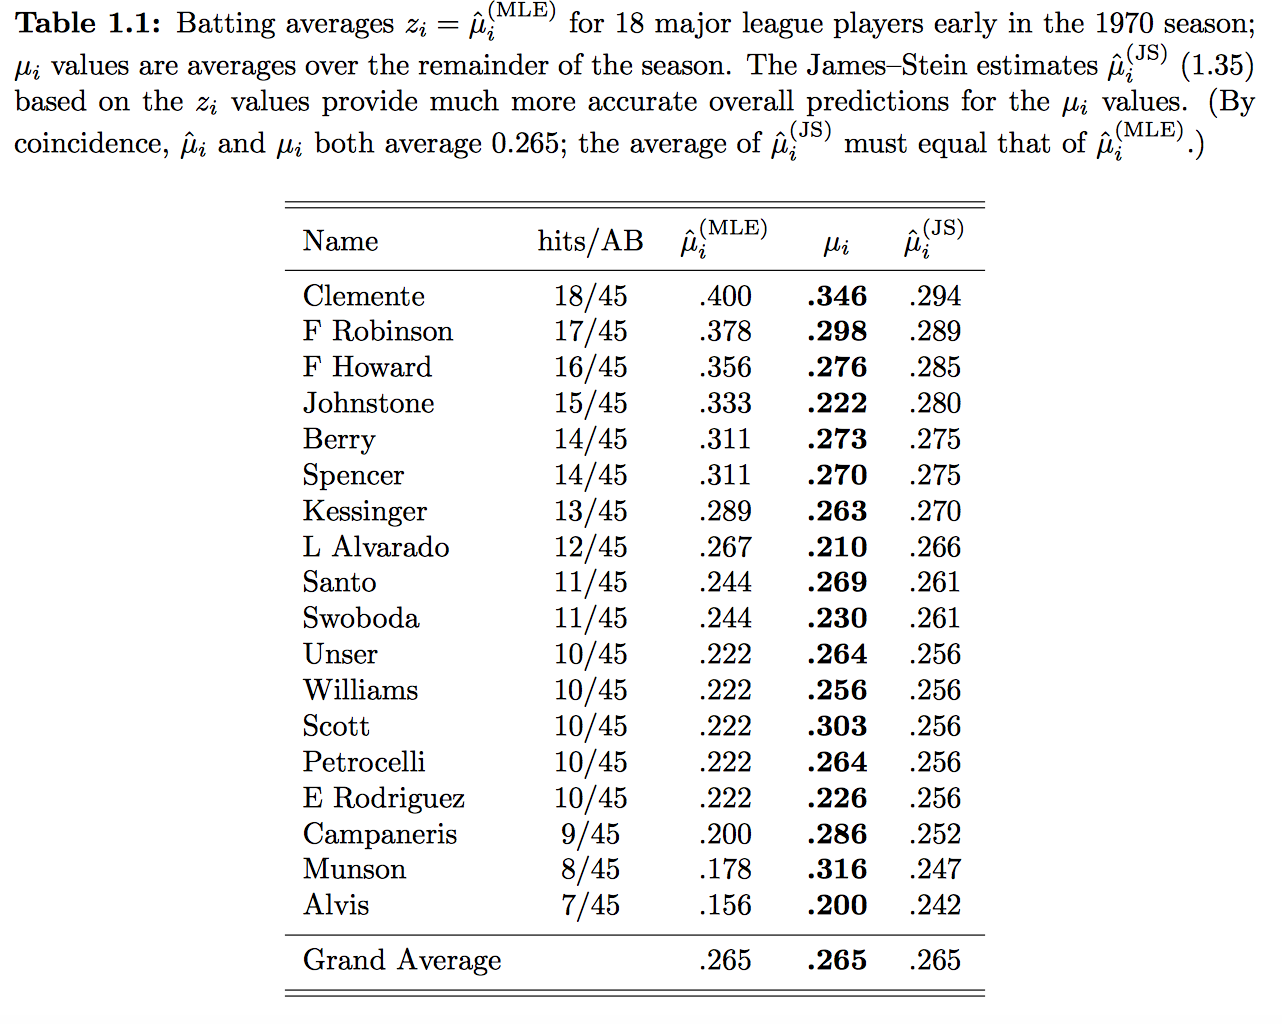
\includegraphics[width=3.5in]{./resources/baseball.png}
\end{center}
\end{frame}

\begin{frame}[fragile]{A (famous) Baseball Example}
Probably we can do better than the MLE here:
\begin{itemize}
\item Thurman Munson wins Rookie of the Year and ends up batting $\mu_i = .316$. If he batted .178 all year, his career would not have lasted long.
\item Clemente's $.400$ seems unlikely to hold up. Last player to hit $> .400$ was Ted Williams $.406$ in 1941.
\item But how?
\end{itemize}
\end{frame}

\begin{frame}[fragile]{Bayesian Shrinkage}
Idea is to take an average between the observed average $y_i$ and the overall mean $\overline{y}$:
\begin{align*}
\widehat{\mu}_i^{JS} &=  (1-\lambda) \cdot \overline{y}  + \lambda \cdot y_i, \quad
\lambda = 1 - \frac{(m-3) \sigma^2}{\sum_i( y_i - \overline{y})^2}
\end{align*}
\begin{itemize}
\item This has the effect of \alert{shrinking} $y_i$ towards the \alert{prior mean} $\overline{y}$.
\item In this case the \alert{prior mean} is just $\overline{y}$ the grand-mean of all players
\item How can information about unrelated players inform us about $\mu_i$?
\item Also consider proportion of foreign cars in Chicago as an additional $y_i$, can this help too?
\item The \alert{shrinkage factor} $\lambda$ depends on sample size and variance, but how is it chosen?
\end{itemize}
\end{frame}



\begin{frame}[fragile]{A Baseball Example}
\begin{center}
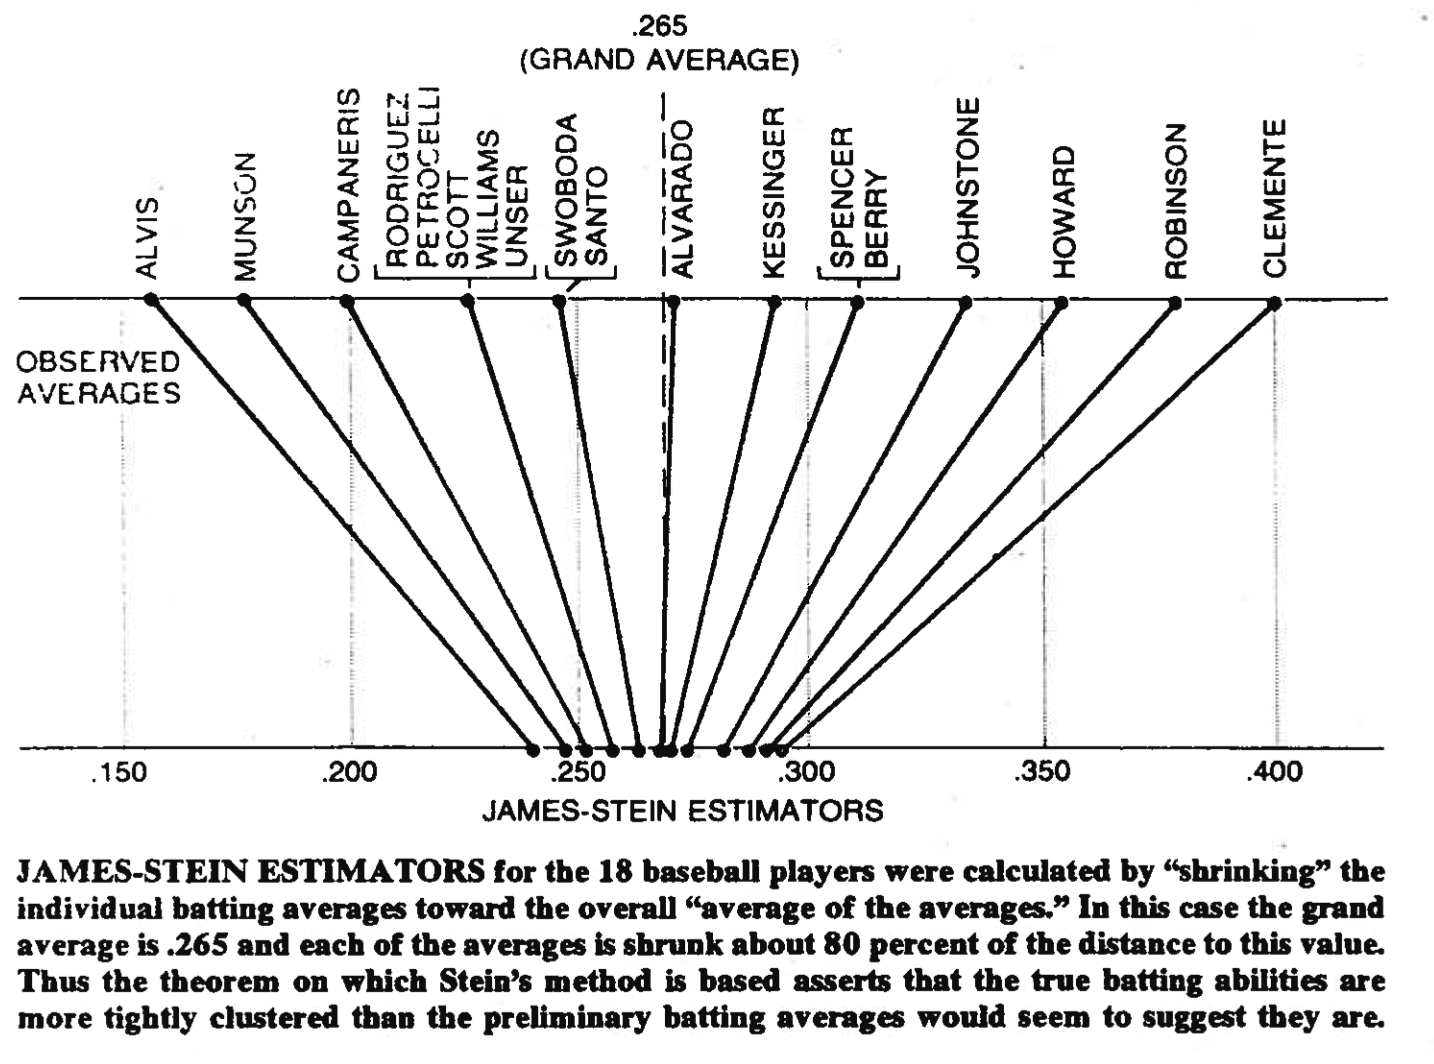
\includegraphics[width=3.5in]{./resources/baseball2.png}
\end{center}
\end{frame}
\section{Example: Diversion Ratios}
\begin{frame}{The Diversion Ratio: Conlon and Mortimer (2018)}
 Raise price of good $j$. People leave. What fraction of leavers switch to $k$?
\begin{eqnarray*}
D_{jk} = \frac{\frac{\partial q_k}{\partial p_j}}{\left|\frac{\partial q_j}{\partial p_j} \right|}
\end{eqnarray*}
It's one of the best ways economists have to characterize competition among sellers.
\begin{itemize}
\item High Diversion: Close Substitutes $\rightarrow$ Mergers more likely to increase prices.
\item Very low diversion $\rightarrow$ products may not be in the same market.\\ (ie: Katz \& Shapiro)
\item Demand Derivatives NOT elasticities.
\item No equilibrium responses.
\end{itemize}
\end{frame}

\begin{frame}
\frametitle{Estimating $\overline{D}_{jk}$}
Remove a product $j$ measure $\Delta q_j$ and $\Delta q_k$.
 \begin{eqnarray*}
 \overline{D_{jk}} =  \frac{\widehat{\Delta q_k}}{|\widehat{\Delta q_j}|} = \frac{ E[q_k | Z=1] - E[q_k | Z=0]}{ \left| E[q_j | Z=1] - E[q_j | Z=0] \right|}  
 =\frac{ E[q_k | Z=1] - E[q_k | Z=0]}{ E[q_j | Z=0] }
 \end{eqnarray*}
\end{frame}

\begin{frame}
\frametitle{Using a Beta-Binomial Prior}
How to restrict $D_{jk} \in [0,1]$?
\begin{eqnarray*}
\Delta q_k | \Delta q_j,D_{jk} &\sim& Bin(n=\Delta q_j, p=D_{jk})\\ \pause
 D_{jk} | \beta_1, \beta_2 &\sim& Beta(\beta_1,\beta_2)\\
E[D_{jk} | \beta_1, \beta_2, \Delta q_j, \Delta q_k] &=& \frac{\beta_1 + \Delta q_k}{\beta_1 + \beta_2 + \Delta q_j}\\ \mu_{jk} &=& \frac{\beta_1}{\underbrace{\beta_1+\beta_2}_{m_{jk}}},  \quad \lambda = \frac{m_{jk}}{m_{jk} + \Delta q_j} \\
\widehat{D_{jk}} &=& \lambda \cdot \mu_{jk} + (1-\lambda) \frac{\widehat{\Delta q_k}}{\widehat{\Delta q_j}}
\end{eqnarray*}
$\mu_{jk}$ is prior mean; $m_{jk}$ is no. pseudo-obs; $\lambda$ weights our prior mean. \\% vs. experimental obs.
When we have a lot of experimental obs, prior receives little weight.
\end{frame}

\begin{frame}
\frametitle{Using a Dirichlet Prior}
How do restrict $D_{j\cdot} \in \Delta$?
\begin{itemize}
\item Same idea as before, but use \alert{Dirichlet Prior}.
\item Acts like pseudo-observations from the \alert{multinomial} distribution.
\item If we had same number of treated observations for each substitute we would have conjugacy/closed form (We don't).
\item Likelihood is $\Delta q_{k} \sim Binomial(\Delta q_j, D_{jk})$ not \alert{multinomial}.
\item We use $m=3.05$ pseudo-observations for the Dirichlet prior.
\item Estimator is still technically \alert{non-parametric}. Why?
\end{itemize}
\end{frame}



\begin{frame}
\frametitle{Shrinkage Estimator, Intuition}
\begin{itemize}
\item We ``shrink'' towards the prior mean when we have experimental estimates that are imprecise.
\item Idea is very simple: when we have lots of data, use the experimental measure.
\item When data are scarce: put more weight on the prior/model-based measure.
\begin{itemize}
\item In practice: FTC/DOJ tend to assume diversion proportional to marketshare
\item Use plain logit (could also use more complicated model)
\item Logit sets the mean of the prior as: $\mu_{jk} = \frac{s_k}{1-s_{j}}$
\end{itemize}
\end{itemize}
\end{frame}

\begin{frame}{Results: Mars }
\tiny
\begin{tabular}{ll |   r r r r  r r r  r}
Firm & Product & \# Weeks & $\Delta q_k$ & $\Delta q_j$ & $\frac{\Delta q_k}{\Delta q_j}$ & Beta(J) & Beta(300) & Dirichlet(4.15)\\ 
\hline  &&\multicolumn{7}{c}{Snickers Removal}\\ \hline
Mars & M\&M Peanut & 176 & 375.52 & -954.30 & 39.35 & 37.04 & 30.80 & 18.40 \\
Mars & Twix Caramel & 134 & 289.60 & -702.39 & 41.23 & 37.86 & 29.49 & 15.88 \\
Pepsi & Rold Gold (Con) & 174 & 161.37 & -900.11 & 17.93 & 16.84 & 13.95 & 7.54 \\
Nestle & Butterfinger & 61 & 72.95 & -362.82 & 20.11 & 17.07 & 11.19 & 4.45 \\
Mars & M\&M Milk Chocolate & 97 & 71.76 & -457.36 & 15.69 & 13.83 & 9.85 & 4.14 \\
Kraft & Planters (Con) & 136 & 78.01 & -759.87 & 10.27 & 9.57 & 7.80 & 3.81 \\
Kellogg & Zoo Animal Cracker & 177 & 65.72 & -970.22 & 6.77 & 6.48 & 5.68 & 2.92 \\
Pepsi & Sun Chip & 159 & 45.30 & -866.09 & 5.23 & 4.98 & 4.33 & 2.07 \\
Hershey & Choc Hershey (Con) & 41 & 29.78 & -179.57 & 16.58 & 12.17 & 6.30 & 2.01 \\
& Outside Good & 180 & 460.89 & -970.22 & 47.50 &  &  & 23.12 \\

\hline  &&\multicolumn{7}{c}{M\&M Peanut Removal}\\ \hline
Mars & Snickers & 218 & 296.58 & -1239.29 & 23.93 & 22.90 & 19.91 & 16.47 \\
Mars & Twix Caramel & 176 & 110.93 & -1014.32 & 10.94 & 10.39 & 8.88 & 6.76 \\
Mars & M\&M Milk Chocolate & 99 & 73.47 & -529.58 & 13.87 & 12.46 & 9.18 & 6.26 \\
Nestle & Raisinets & 181 & 71.82 & -1001.14 & 7.17 & 6.82 & 5.82 & 4.37 \\
Kraft & Planters (Con) & 190 & 61.42 & -1046.10 & 5.87 & 5.62 & 4.90 & 3.60 \\
Hershey & Twizzlers & 62 & 32.98 & -332.99 & 9.90 & 8.32 & 5.32 & 3.35 \\
Kellogg & Rice Krispies Treats & 46 & 22.37 & -220.17 & 10.16 & 7.90 & 4.43 & 2.51 \\
Pepsi & Frito  & 160 & 37.25 & -902.42 & 4.13 & 3.95 & 3.47 & 2.37 \\
& Outside Good& 218 & 606.18 & -1238.49 & 48.95 &  &  & 36.35 \\
\end{tabular}
\end{frame}


\begin{frame}{Results: Kellogg's}
\tiny
\begin{tabular}{ll |   r r r r  r r r  r}
Firm & Product & \# Weeks & $\Delta q_k$ & $\Delta q_j$ & $\frac{\Delta q_k}{\Delta q_j}$ & Beta(J) & Beta(300) & Dirichlet(4.15)\\ 
\hline  &&\multicolumn{7}{c}{Animal Crackers Removal}\\ \hline
Pepsi & Rold Gold (Con) & 132 & 114.39 & -440.80 & 25.95 & 22.90 & 16.21 & 9.89 \\
Mars & Snickers & 145 & 92.44 & -483.63 & 19.11 & 17.26 & 13.04 & 7.58 \\
Mars & M\&M Peanut & 142 & 77.72 & -469.44 & 16.55 & 14.98 & 11.43 & 6.47 \\
Kellogg & CC Famous Amos & 144 & 66.18 & -478.20 & 13.84 & 12.40 & 9.15 & 5.39 \\
Pepsi & Baked Chips (Con) & 134 & 62.55 & -447.60 & 13.97 & 12.46 & 9.13 & 5.27 \\
Mars & Twix Caramel & 110 & 50.17 & -338.97 & 14.80 & 12.75 & 8.74 & 4.58 \\
Sherwood & Ruger Wafer (Con) & 119 & 48.20 & -368.65 & 13.07 & 11.28 & 7.63 & 4.28 \\
Hershey & Choc Herhsey (Con) & 30 & 33.60 & -132.57 & 25.34 & 17.14 & 7.86 & 3.81 \\
Kellogg & Rice Krispies Treats & 13 & 23.52 & -37.80 & 62.22 & 23.24 & 7.16 & 2.99 \\
Kar's Nuts & Kar Sweet\&Salty Mix & 95 & 30.06 & -334.50 & 8.99 & 7.72 & 5.27 & 2.73 \\
Misc & Popcorn (Con) & 56 & 25.72 & -226.89 & 11.34 & 8.92 & 5.08 & 2.61 \\
Kraft & Planters (Con) & 114 & 28.05 & -380.25 & 7.38 & 6.53 & 4.78 & 2.43 \\
Mars & M\&M Plain & 73 & 22.67 & -295.07 & 7.68 & 6.47 & 4.26 & 2.15 \\
& Outside Good& 145 & 240.52 & -482.91 & 49.81 &  &  & 21.98 \\

\hline  &&\multicolumn{7}{c}{Famous Amos Removal}\\ \hline
Pepsi & Sun Chip & 139 & 143.60 & -355.68 & 40.37 & 34.39 & 22.66 & 15.75 \\
Kraft & Planters (Con) & 121 & 82.11 & -332.61 & 24.69 & 20.89 & 13.68 & 8.75 \\
Hershey & Choc Hershey (Con) & 38 & 48.60 & -66.84 & 72.72 & 36.93 & 13.36 & 7.18 \\
Pepsi & Frito & 119 & 49.88 & -313.21 & 15.93 & 13.44 & 8.85 & 5.32 \\
Misc & Rasbry Knotts & 133 & 46.62 & -345.38 & 13.50 & 11.45 & 7.49 & 4.81 \\
Pepsi & Grandmas Choc Chip & 95 & 39.99 & -259.21 & 15.43 & 12.51 & 7.62 & 4.49 \\
Pepsi & Dorito Buffalo Ranch & 72 & 38.11 & -224.24 & 17.00 & 13.28 & 7.53 & 4.43 \\
Pepsi & Chs PB Frito Cracker & 34 & 26.87 & -83.65 & 32.13 & 18.16 & 7.14 & 3.74 \\
Kellogg & Choc Sandwich FA & 57 & 27.97 & -122.04 & 22.91 & 15.06 & 6.84 & 3.69 \\
Pepsi & Rold Gold (Con) & 147 & 32.62 & -392.22 & 8.32 & 7.40 & 5.54 & 3.19 \\
Kraft & Oreo Thin Crisps & 29 & 20.73 & -43.29 & 47.89 & 19.20 & 6.12 & 3.05 \\
Mars & Combos (Con) & 98 & 23.56 & -274.54 & 8.58 & 7.03 & 4.34 & 2.61 \\
& Outside Good& 156 & 192.90 & -399.12 & 48.33 &  &  & 20.95 \\
\end{tabular}
\end{frame}

\begin{frame}{Comparison of Assumptions: Snickers Experiment}
\begin{table}
\footnotesize
\begin{tabular}{|l|ccccc|}
%& Total  & Impose & Impose & Impose & Impose\\ 
\multicolumn{1}{c}{} & \multicolumn{1}{c}{Total} & \multicolumn{1}{c}{Assn 1} & \multicolumn{1}{c}{Assn 2}   & \multicolumn{1}{c}{Assn 3} & \multicolumn{1}{c}{Assn 4} \\ 
\multicolumn{1}{c}{} 	&\multicolumn{1}{c}{} 	&\multicolumn{1}{c}{} 	&\multicolumn{1}{c}{} 	&\multicolumn{1}{c}{($m = K$)} 	&\multicolumn{1}{c}{(m = 4.15)} \\ \hline
Products with $D_{jk} < $ 0 & 51&24&26&0&0\\
Products with $0 \leq D_{jk} \leq 10$& 51&13&15&43&48\\
Products with $10 \leq D_{jk} \leq 20$ & 51&5&5&5&2\\
Products with $D_{jk} > $ 20 & 51&9&5&3&1\\ \hline
Sum of all positive $D_{jk}$s & 51&402.84&301.95&265.41&98.72\\
Sum of all negative $D_{jk}$s & 51&-238.90&-239.07&0.00&0.00\\
\hline
\end{tabular}\\
\footnotesize
Note: Table includes only products for which there were at least 50 sales of the focal product in control weeks, on average.
\end{table}
\end{frame}


\begin{frame}[fragile]{Stan Code}
\footnotesize
\begin{verbatim}
% Main Specification: Dirichlet Prior
data {
  int<lower=1> J;               // number of products, including outside good
  int<lower=1> N[J];            // number of trials
  int<lower=0> y[J];            // number of successes for each product j
  vector[J] priors;    // mean of the distribution of alpha
}

parameters {
  simplex[J] theta;
}

model {
  theta ~ dirichlet(priors);
  for (j in 1:J) {
    y[j] ~ binomial(N[j], theta[j]);
  }
}
\end{verbatim}
\end{frame}


\section{Bayesian Estimation}

\begin{frame}{How do we estimate these models?}
A few options
\begin{itemize}
\item With conjugate priors we can closed forms
\item Can do it by hand if we have \alert{sufficient statistics}
\begin{itemize}
\item Clear in beta-binomial or poisson-gamma relationship.
\item Mostly not the case.
\end{itemize}
\item Mostly we do what is known as \alert{Markov Chain Monte Carlo}
\item The goal is to draw from $f(\theta | \mathbf{X})$ or to compute moments of the distribution $E_f[g(\theta)]$.
\end{itemize}
\end{frame}

\begin{frame}{Monte Carlo Methods}
\begin{itemize}
\item Suppose we want to calculate a function 
$$E_f[g(x)] = \int g(x) f(x) d\,x$$
\item How do we do it?
\begin{enumerate}
\item Draw from $\hat{x}_s \sim f(x)$
\item Caclulate $g(\hat{x}_s)$
\item Repeat for $s=1\ldots,S$
\item Calculate $E[\hat{g}]=\frac{1}{S} \sum_{s=1}^S g(\hat{x}_s)$
\end{enumerate}
\end{itemize}
\end{frame}


\begin{frame}[fragile]{Monte Carlo Example}
\begin{itemize}
\item Let's integrate $g(x) = \phi(x)$ (normal pdf) over $f(x) = Unif(0,1)$ from $[0,1]$.
\item We know the answer is $\Phi(1) - \Phi(0)$.
\end{itemize}
\begin{minted}{R}
Integral <- function(n){
    X <- runif(n)
    Y <- exp(-X^2/2)/sqrt(2*pi)
    Int <- sum(Y)/n
    Error <- Int-(pnorm(1)-pnorm(0))
    list(Int,Error)}
\end{minted}

\end{frame}



\begin{frame}{Gibbs Sampling}
The first building block is known as \alert{Gibbs Sampling}
\begin{itemize}
\item Suppose that $p(x,y)$ is a p.d.f or p.m.f that is hard to sample directly from.
\item But suppose that $p(x | y)$ or $p(y | x)$ are easy to sample from.
\item Gibbs sampler says:
\begin{enumerate}
\item Initialize $(x_0,y_0)$.
\item Randomly draw $y_1 \sim g(y | x_0)$.
\item Randomly draw $x_1 \sim f(x | y_1)$.
\item Randomly draw $y_2 \sim g(y | x_1)$.
\item Rinse and Repeat. 
\end{enumerate}
\item This sequence $(x_0,y_0),(x_1,y_1), (x_2,y_2), \ldots$ is a \alert{Markov Chain}.
\item Why? Because $(x_k,y_k) | (x_{k-1},y_{k-1})$ doesn't depend on $x_{k-h}$ or $y_{k-h}$ for $h \geq 2$.
\begin{itemize}
\item This does not mean that $(x_3,y_3)$ and $(x_1,y_1)$ are I.I.D!
\end{itemize}
\end{itemize}
\end{frame}

\begin{frame}{Gibbs Sampler: Example}
\end{frame}

\begin{frame}{Metropolis Hastings}
\end{frame}

\begin{frame}{Metropolis Hastings: Example}
\end{frame}

\section*{Thanks!}
\end{document}

\item We probably are interested in more observations $[x_1,\ldots,x_n]$ instead of just $x_1$.
\item $\sum_{i=1}^N x_i \sim Bin(N,p)$.